\documentclass[10pt,a4paper]{article}
\usepackage[margin=1in]{geometry}
\usepackage{tikz}
\usepackage{fontspec}
\usepackage{xcolor}

\definecolor{accent}{RGB}{60, 60, 60}
\definecolor{lightgray}{RGB}{180, 180, 180}

\begin{document}
\thispagestyle{empty}

% Background decorative elements

\begin{tikzpicture}[overlay, remember picture]
    % Top accent line
    \draw[line width=3pt, color=black] 
        ([yshift=-2.5cm]current page.north west) -- 
        ([yshift=-2.5cm]current page.north east);
    
    % Bottom accent line
    \draw[line width=2pt, color=black] 
        ([yshift=2.5cm]current page.south west) -- 
        ([yshift=2.5cm]current page.south east);
    
    % Side decorative bar
    \fill[black] 
        ([xshift=1.5cm, yshift=-3.5cm]current page.north west) 
        rectangle 
        ([xshift=1.7cm, yshift=3.5cm]current page.south west);
    
    % Subtle corner squares
    \fill[black] ([xshift=2cm, yshift=-2.8cm]current page.north west) rectangle ++(0.4, -0.4);
    \fill[black] ([xshift=2cm, yshift=2.8cm]current page.south west) rectangle ++(0.4, 0.4);
    \fill[black] ([xshift=-2.4cm, yshift=-2.8cm]current page.north east) rectangle ++(-0.4, -0.4);
    \fill[black] ([xshift=-2.4cm, yshift=2.8cm]current page.south east) rectangle ++(-0.4, 0.4);
    
    % Light geometric elements
    \draw[color=lightgray, line width=0.5pt, dashed] 
        (3, -5) -- (15, -5);
    \draw[color=lightgray, line width=0.5pt, dashed] 
        (3, -18) -- (15, -18);
\end{tikzpicture}

\vspace*{2.5cm}

% Title Section
\begin{center}
    {\fontsize{42}{50}\selectfont \textbf{ECONOMICS}}\\[0.8cm]
    {\fontsize{18}{22}\selectfont \textcolor{accent}{COMPREHENSIVE COURSE NOTES}}\\[2.5cm]
    
    % Decorative line
    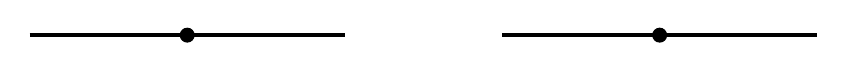
\begin{tikzpicture}
        \draw[line width=1.5pt] (0,0) -- (4,0);
        \filldraw (2,0) circle (2.5pt);
        \draw[line width=1.5pt] (6,0) -- (10,0);
        \filldraw (8,0) circle (2.5pt);
    \end{tikzpicture}
    \vspace{2cm}
    
    % Topics Covered
    {\fontsize{12}{16}\selectfont \textbf{Topics Included:}}\\[0.5cm]
    
    \begin{tabular}{p{5.5cm} p{5.5cm}}
        \textbullet\ Basic Economic Concepts & \textbullet\ Demand \& Supply \\
        \textbullet\ Elasticity of Demand \& Supply & \textbullet\ Consumer Behavior \& Utility \\
        \textbullet\ Indifference Curve Analysis & \textbullet\ Production \& Cost \\
        \textbullet\ Firm Decisions \& Revenue & \textbullet\ Market Structures \\
        \textbullet\ Macroeconomics & \textbullet\ Investment Appraisal \\
    \end{tabular}
    
    \vspace{2cm}
    
    % Decorative line
    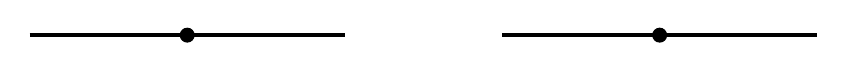
\begin{tikzpicture}
        \draw[line width=1.5pt] (0,0) -- (4,0);
        \filldraw (2,0) circle (2.5pt);
        \draw[line width=1.5pt] (6,0) -- (10,0);
        \filldraw (8,0) circle (2.5pt);
    \end{tikzpicture}
    \vspace{1.5cm}
    
    % Course Information
    {\fontsize{11}{14}\selectfont \textcolor{accent}{Two-Column Format | Black \& White | LaTeX Typesetting}}\\[0.3cm]
    {\fontsize{11}{14}\selectfont \textcolor{accent}{Definitions | Memory Triggers | Mathematical Derivations | Graphs}}\\[0.3cm]
    {\fontsize{11}{14}\selectfont \textcolor{accent}{Case Studies | Exam Questions \& Model Answers}}\\[2cm]
    
    % Bottom decorative bar
    \vspace*{\fill}
    \begin{tikzpicture}[overlay, remember picture]
        \fill[black] 
            ([xshift=1.5cm, yshift=1cm]current page.south west) 
            rectangle 
            ([xshift=-1.5cm, yshift=1.3cm]current page.south east);
        \node[text=white, font=\small] 
            at ([yshift=1.15cm]current page.south) 
            {Academic Year 2025--2026};
    \end{tikzpicture}
    
    \vspace*{0.5cm}
    \hfill {\fontsize{10}{12}\selectfont \textit{Compiled using \LaTeX}}
    
\end{center}

\end{document}